\documentclass[11pt]{article}
%\usepackage{psfig}
\usepackage{graphicx}
\usepackage{enumitem}
\usepackage{amsmath,amssymb,amsthm,listings,hyperref}
\usepackage{tikz}
\usepackage{latexsym}
\usepackage{amsfonts}

\title{CS 4641 Project 2 Report}
\author{HU Heng}
\date{March 2, 2019}
\begin{document}
\maketitle
\section{Overview}
This report is for CS 4641 Machine Learning project 2 Randomized Optimization. In the following pages, you will see analysis of neural network which updates weights by randomized optimization instead of back propagation. I will show the results by some figures which is about the performance of each randomized optimization algorithm. In addition, I will introduce three problems that can be solved by randomized optimization. \\
\\
For first part of the project that is train neural network using randomized optimization algorithms, I use mlrose. For the second part of the project, I use ABAGAIL.

\section{Datasets}
The datasets I choose is adult dataset which is one of the datasets I used in project 1. Adult dataset is extracted from the 1994 Census database. There are 14 attributes and the result is whether the income is greater than \$50k or not. It is a binary classification problem and there are 48842 instances in total. I believe there should be enough data to train a good model using different algorithms. In addition, binary classification problem is not complicated and it would be suitable for training.

\section{Train Neural Network by Randomized Optimization Algorithm}

\begin{figure}[h!]
  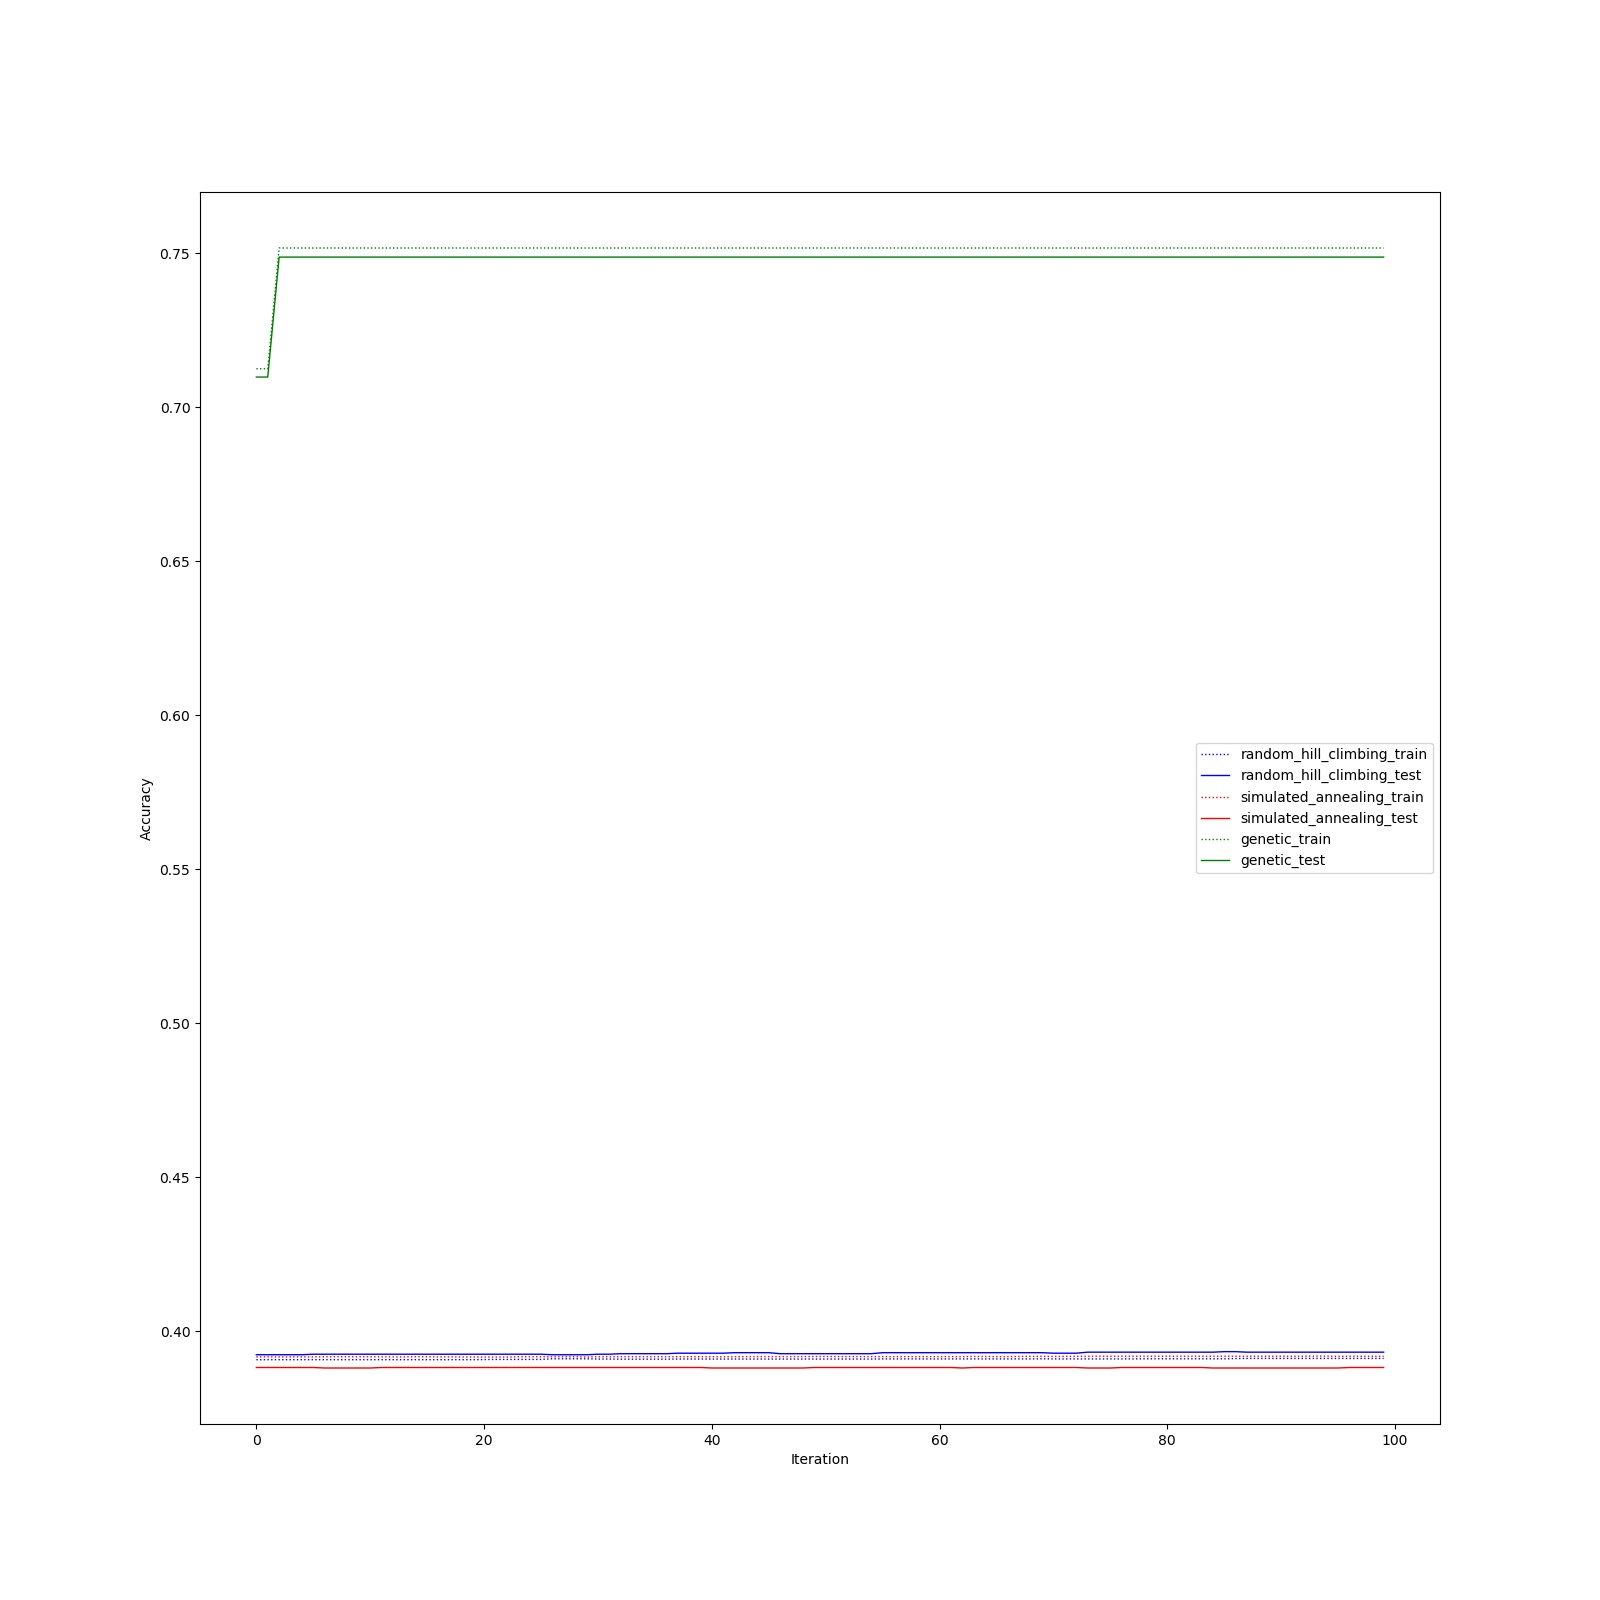
\includegraphics[width=\linewidth]{../plot/nn_plot.jpg}
  \caption{The Performance of Different Training Algorithms}
  \label{fig:nn}
\end{figure}

\begin{table}[h!]
  \begin{center}
    \caption{Hyperparameters}
    \label{tab:hy_nn}
    \begin{tabular}{l|l}
      \textbf{Algorithm} & \textbf{Hyperparameters}\\
      \hline
      Random Hill Climbing & \\
      Simulated Annealing &  start temperature: 1E12, cooling exponent: .99\\
      Genetic & population size: 200, mutation probability: 0.1\\
    \end{tabular}
  \end{center}
\end{table}

\begin{table}[h!]
  \begin{center}
    \caption{Performance of Algorithms}
    \label{tab:adult}
    \begin{tabular}{l|c}
      \textbf{Training Algorithm} & \textbf{Testing Accuracy}\\
      \hline
      Random Hill Climbing & 44.06\%\\
      Simulated Annealing & 44.05\%\\
      Genetic Algorithm & 75.43\%\\
      Gradient Descent & 78.86\%\\
    \end{tabular}
  \end{center}
\end{table}


Fig.\ref{fig:nn} shows the performance of neural network using different training algorithms, Table.\ref{tab:hy_nn} shows the hyperparameters for three algorithms and Table.\ref{tab:adult} shows the performance of different training algorithms on test data. We can see that if we use random hill climbing or simulated annealing to train the neural network, the accuracy almost keep the same. The accuracy converges and is even worse than random guess, which is obviously underfitting. Using genetic algorithm to train neural network seems to perform well. The accuracy converges within ten iterations and there is no overfitting. The accuracies for using genetic algorithm and gradient descent are close to each other. So I believe training neural network using genetic algorithm is a good alternative. It reduces training time while preserving the testing accuracy. Also, no need to worry about overfitting.\\
\\
There must be some underlying reasons for getting that result. Consider this problem: What does it mean to apply randomized algorithms on neural network weights? For gradient descent, our goal is to minimize the gradient by back propagation. So the fitness function should describe how our data is fit with neural network model and our algorithms will optimize that fitness function by adjusting the weight of neural network. Now things become clear, since there are 14 attributes, I believe the fitness function is a complicated one and there are many peaks, that is many local optimas. Random hill climbing will hang around local optimas obviously. Simulated annealing may step back and go other directions but as time goes by, it will still be caught by local optimas. While for genetic algorithm, since the fitness function is clear(it should be something similar to gradient), genetic algorithm can find that value quickly. For the first several iterations, it is actually evolve to the desired weights of neural network.

\section{Randomized Optimization Problems}
\subsection{Traveling Salesman Problem}
Traveling Salesman problem is a very famous NP-hard problem which asks the following question: "Given a list of cities and the distances between each pair of cities, what is the shortest possible route that visits each city and returns to the origin city?" Though it is a NP-hard problem, there are heuristics algorithms and randomized algorithms may also reach a close solution. Genetic algorithm performs the best among the four randomized algorithms. It takes fewer iterations to get better result.
\begin{figure}[h!]
  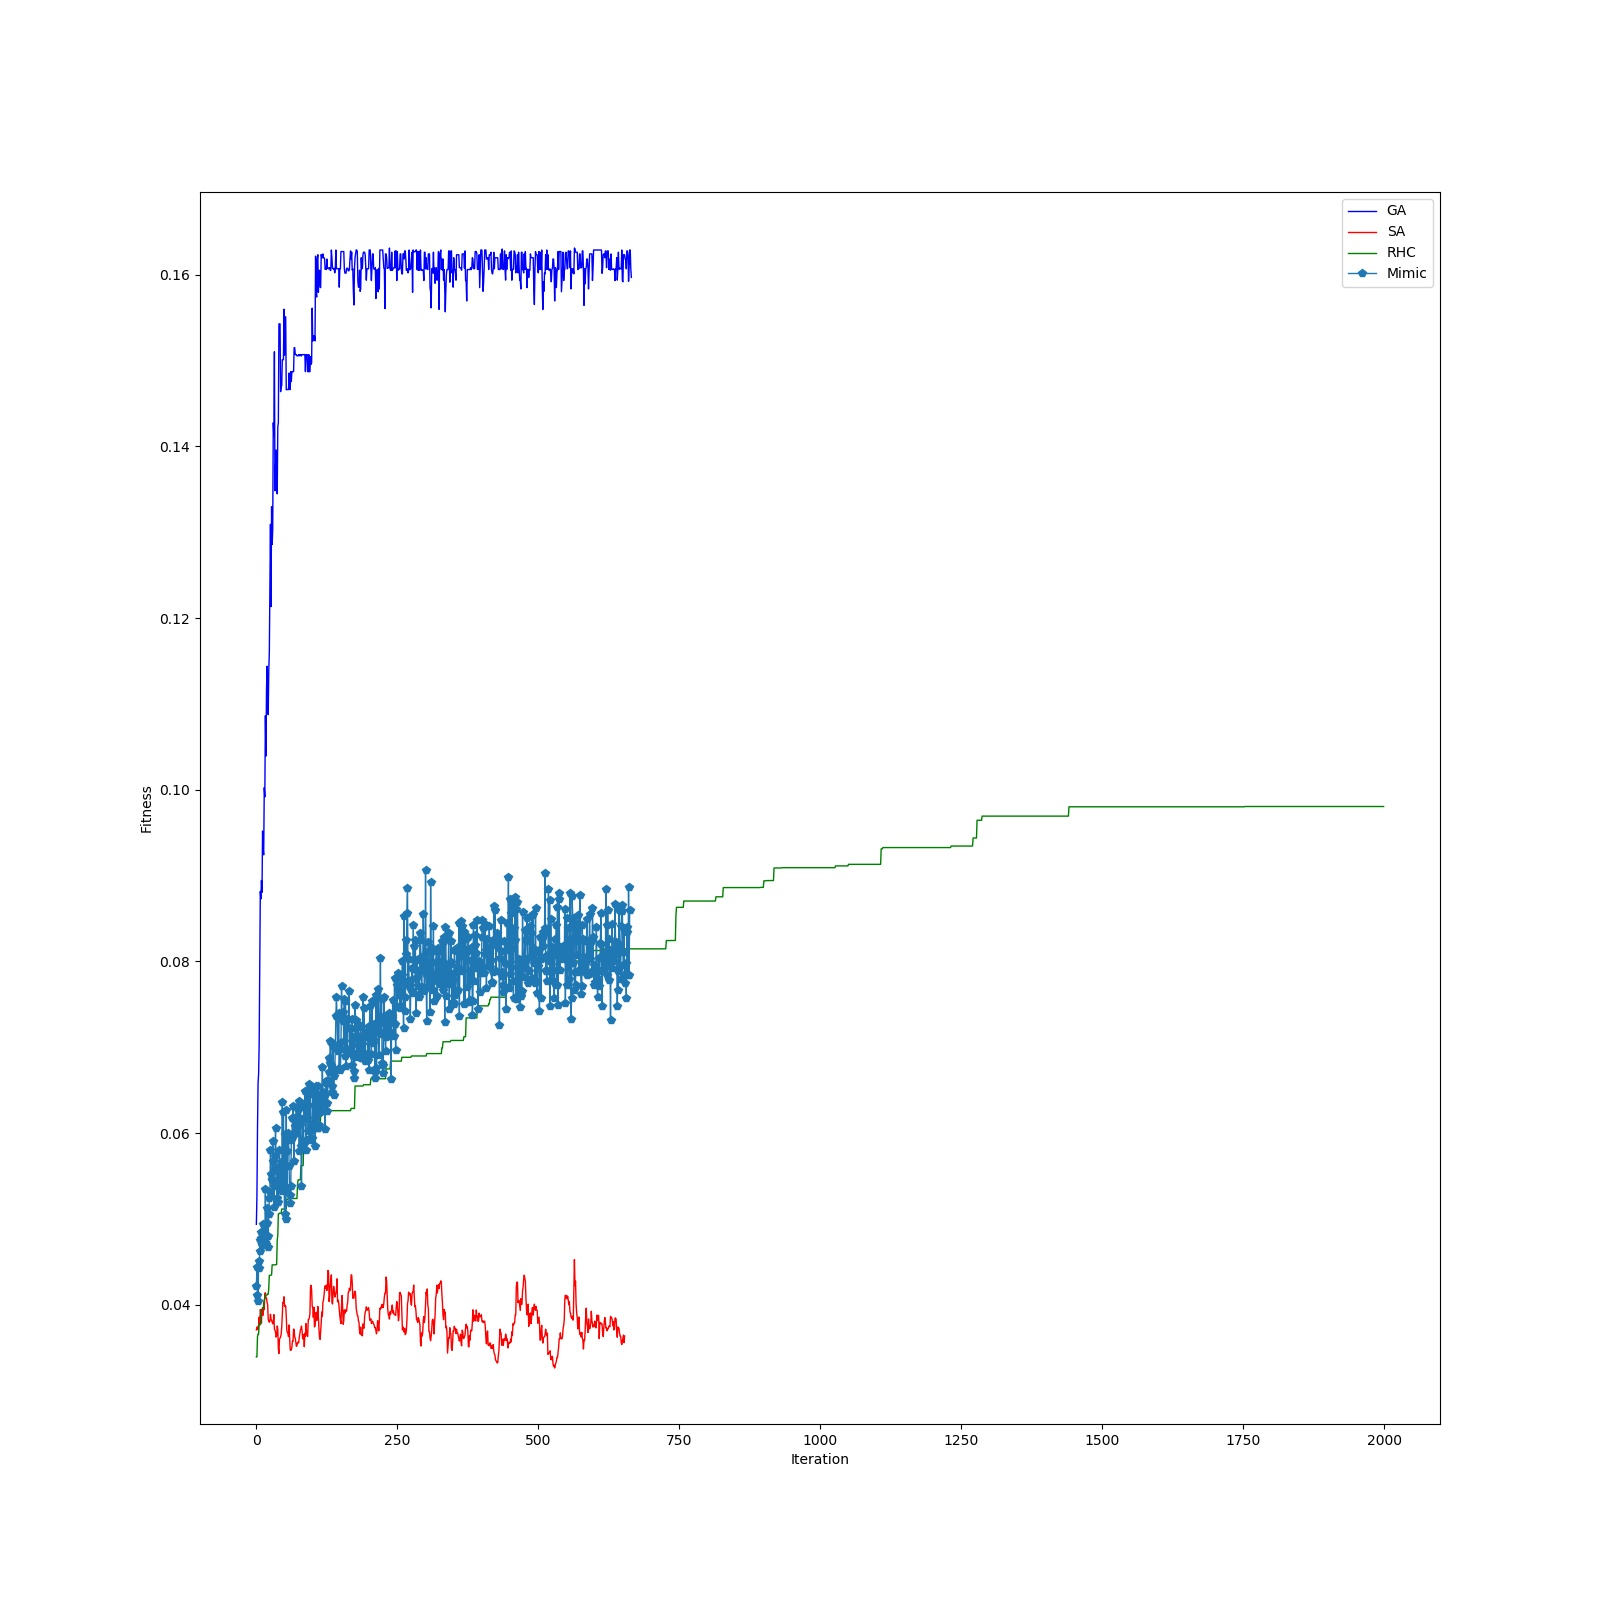
\includegraphics[width=\linewidth]{../plot/ts_plot.jpg}
  \caption{The performance of Algorithms on Traveling Salesman}
  \label{fig:ts}
\end{figure}
\\Fig.\ref{fig:ts} shows the learning curve of each algorithm and Table. It is clear that Genetic algorithm performs much better than other three algorithms. Simulated annealing has the worst performance. Based on the graph, we may conclude that for simulated annealing, the man is actually going up and down again and again but he actually has no improvement. While random hill climbing is actually going to somewhere better. I believe this is because there exists multiple peaks and simulated annealing always steps back and hence get stuck and the original point while random hill climbing will not step back so it performs better than simulated annealing. Generic algorithm fits this problem better because you know your fitness function very clearly. Then, genetic algorithm can reach a good solution in short time.\\
\\Table.\ref{tab:hy_ts} shows the hyperparameters for the four algorithms. (Random hill climbing has no hyperparameters)
\begin{table}[h!]
  \begin{center}
    \caption{Hyperparameters}
    \label{tab:hy_ts}
    \begin{tabular}{l|l}
      \textbf{Algorithm} & \textbf{Hyperparameters}\\
      \hline
      Random Hill Climbing & \\
      Simulated Annealing &  start temperature: 1E12, cooling exponent: .95\\
      Genetic & population size: 200, number to mate: 150, number to mutate: 20\\
      MIMIC & sample size:200, samples to keep:10\\
    \end{tabular}
  \end{center}
\end{table}

\subsection{Countones}
\begin{figure}[h!]
  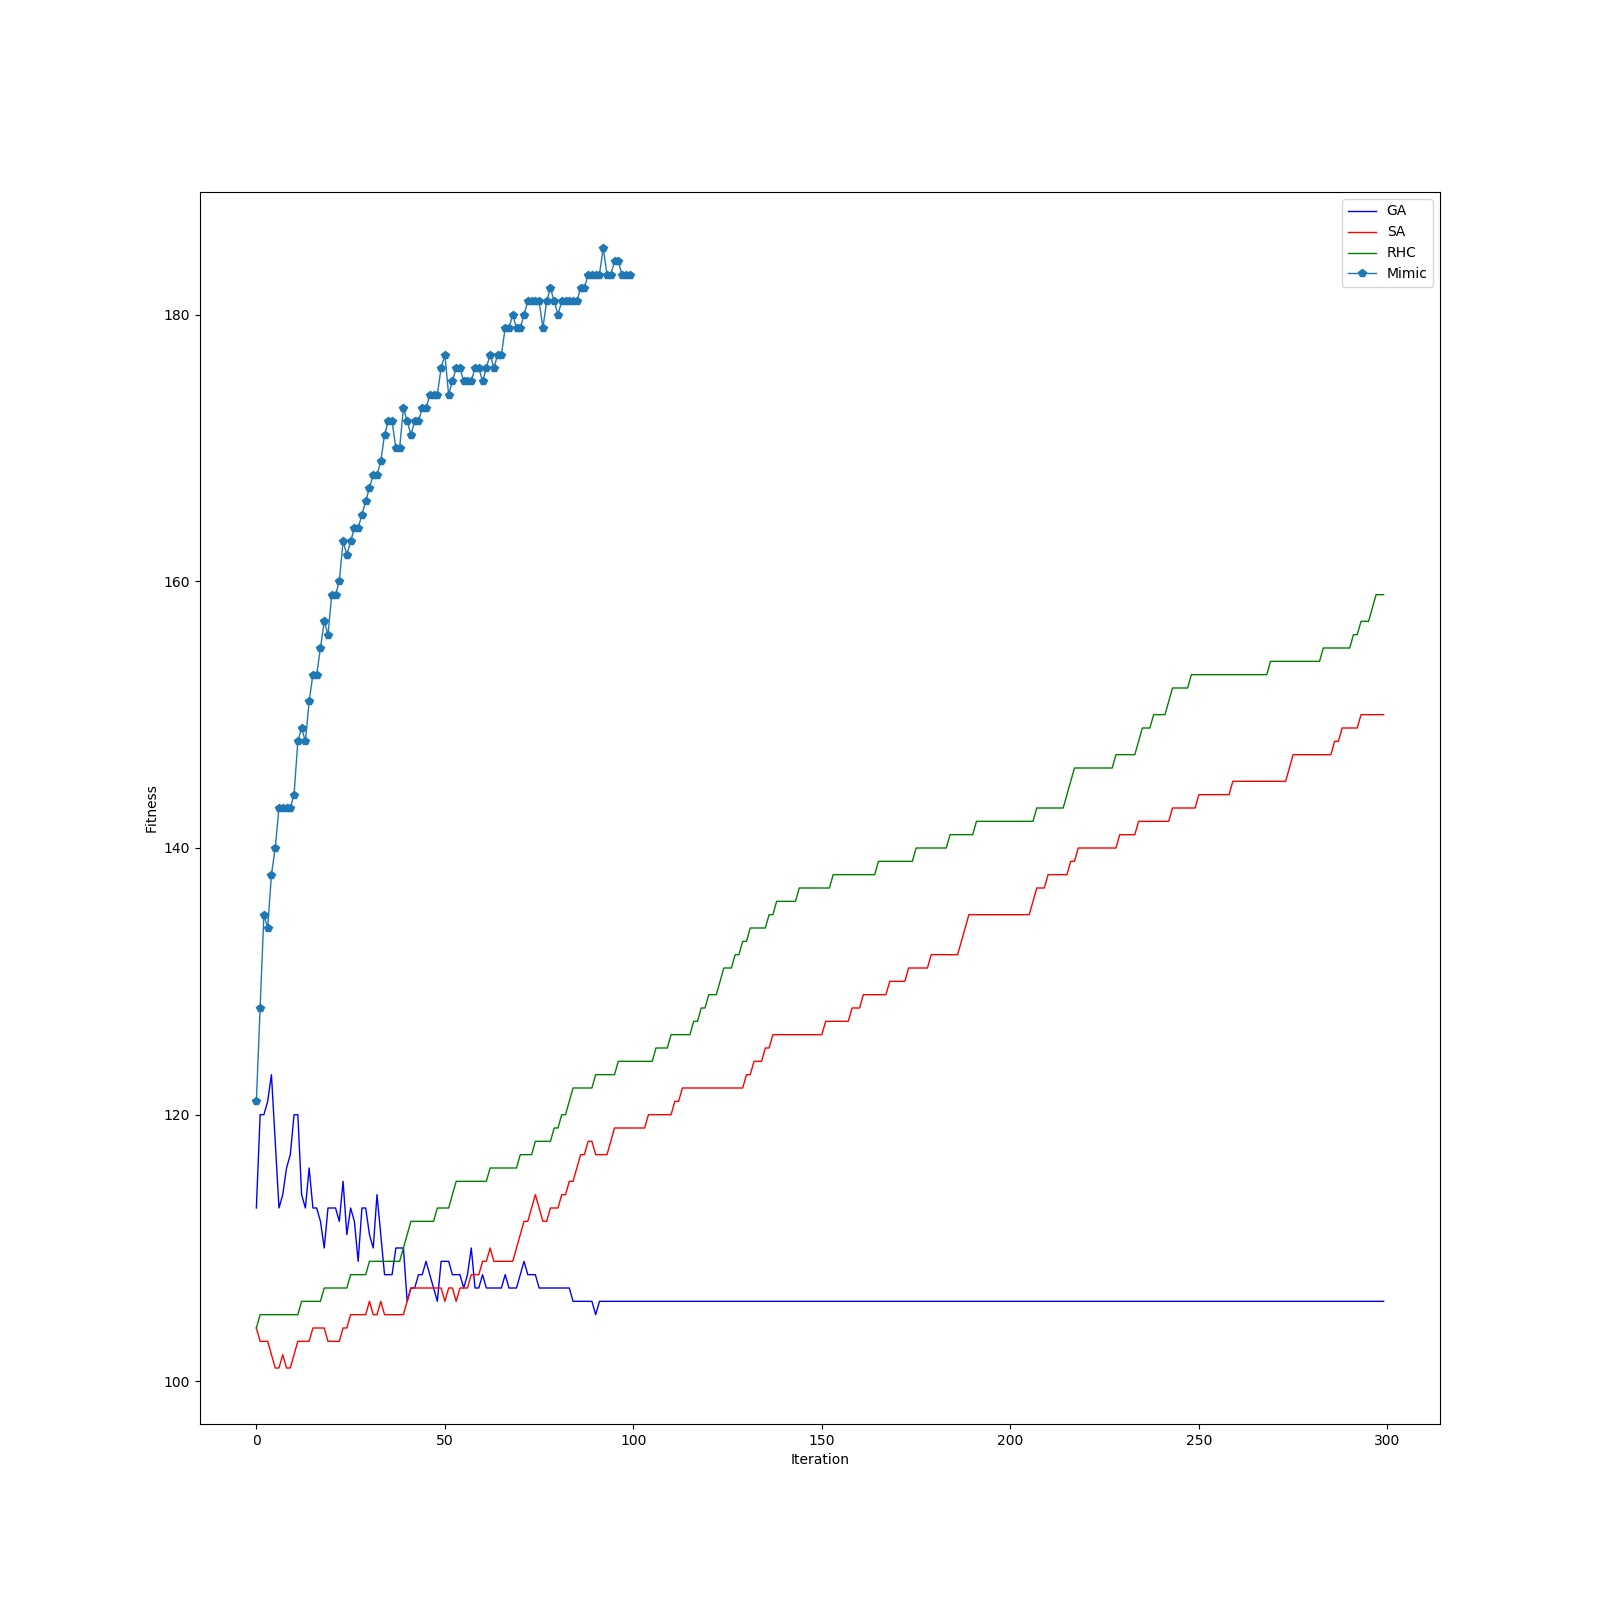
\includegraphics[width=\linewidth]{../plot/countones_plot.jpg}
  \caption{The performance of Algorithms on Countones}
  \label{fig:countones}
\end{figure}
Countones problem asks us to find the number of "one"s in a bitstring. Fig.\ref{fig:countones} shows the performance of each algorithm. MIMIC has the best performance among the algorithms. It will have a better solution in shorter iterations. Since countones is not a very complex problem, random hill climbing and simulated annealing perform well, they all can find the optima after enough time. In addition, they have similar performance, which is reasonable since these two algorithms are actually very similar except that simulated annealing can step back with some probability. The interesting thing is that simulated annealing does slightly worse compared with random hill climbing. Here goes my explanation. At the very beginning, the fitness goes down because it choose to step back when temparature is high. This leads to a wrong direction and after some steps, it goes back to the correct way and go along the path later. So the curve looks like move the curve of random hill climbing. Another interesting observation is that genetic algorithm is getting worse and it even converges! I believe my choice of hyperparameter can help explain it. In my choice of hyperparameter, everyone is goint to mate and noone is to mutate. Then after many iterations, the "bad" ones dominates! My conclusion is that it is really important to have mutation both in choosing hyperparameters and in real world. MIMIC can reach a higher fitness value within shorter iterations. To be honest, I am confused with it. Since MIMIC focus more on the sturcture of the problem, it may suggest that previous examples contains much information, which makes me confused.\\
\\Table.\ref{tab:hy_count} shows the hyperparameters for the four algorithms. (Random hill climbing has no hyperparameters)
\begin{table}[h!]
  \begin{center}
    \caption{Hyperparameters}
    \label{tab:hy_count}
    \begin{tabular}{l|l}
      \textbf{Algorithm} & \textbf{Hyperparameters}\\
      \hline
      Random Hill Climbing & \\
      Simulated Annealing &  start temperature: 100, cooling exponent: .95\\
      Genetic & population size: 20, number to mate: 20, number to mutate: 0\\
      MIMIC & sample size:50, samples to keep:10\\
    \end{tabular}
  \end{center}
\end{table}


\subsection{Flipflop}
\begin{table}[h!]
  \begin{center}
    \caption{Hyperparameters}
    \label{tab:hy_ff}
    \begin{tabular}{l|l}
      \textbf{Algorithm} & \textbf{Hyperparameters}\\
      \hline
      Random Hill Climbing & \\
      Simulated Annealing &  start temperature: 100, cooling exponent: .95\\
      Genetic & population size: 200, number to mate: 100, number to mutate: 20\\
      MIMIC & sample size:200, samples to keep: 5\\
    \end{tabular}
  \end{center}
\end{table}
\begin{figure}[h!]
  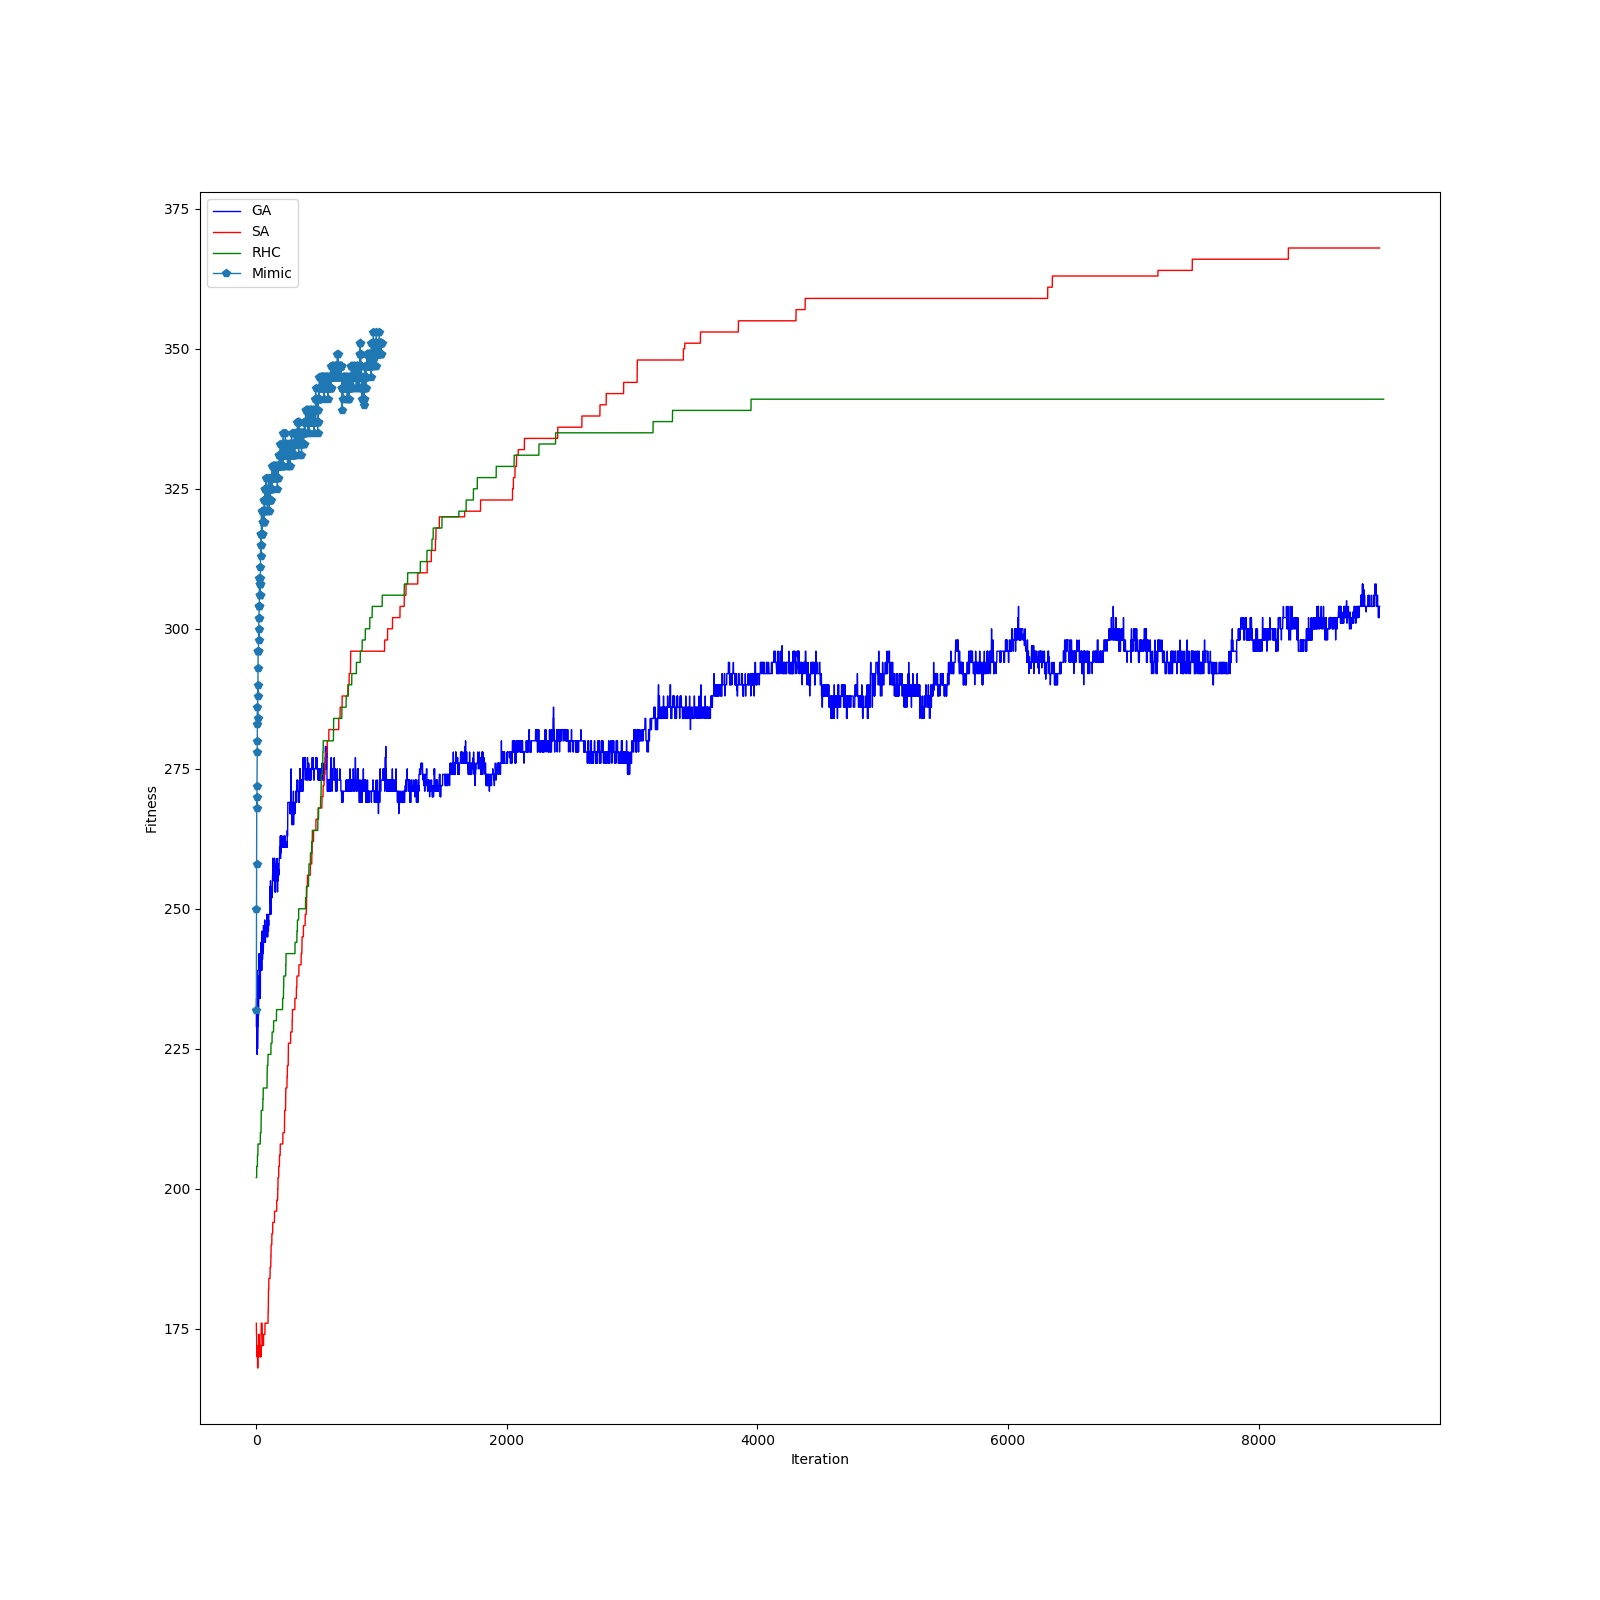
\includegraphics[width=\linewidth]{../plot/ff_plot.jpg}
  \caption{Performance of Algorithms on Flipflop}
  \label{fig:ff}
\end{figure}
Flipflop problem asks us to find the number of alternating bits in a bitstring. Simulated annealing fits this problem very well. Fig.\ref{fig:ff} shows the performance of four algorithms. At this time, genetic algorithm is the worst one, random hill climbing will converge to somewhere worse than simulated annealing and MIMIC works better than random hill climbing but worse than simulated annealing. The reason for difference between random hill climbing and simulated annealing is clear. The flipflop problem has several peaks and it is not strange for random hill climbing to get stuck at some local optima. For simulated annealing, it has some probability to jump out of the local optima, so it gets a better performance. Genetic algorithm has a bad performence probably because many bitstrings can have the same flipflop value, which makes genetic algorithm confused. \\
\\Table.\ref{tab:hy_ff} shows the hyperparameters for the four algorithms. (Random hill climbing has no hyperparameters)

\subsection{Summary}
Table.\ref{tab:all} shows the best algorithm for each problem I introduce. Genetic algorithm fits the problems which have a very clear fitness function. It can give a good solution for traveling salesman problem in reasonable time. Random hill climbing and simulated annealing are two similar algorithms. The difference is that simulated annealing allows step back in the beginning. So when the problem space is simple and local optima is the global optima, these two algorithms can get the correct solution and random hill climbing will have a shorter run time. When there exists multiple local optimas, random hill climbing should not be used because it has a high probability to get stuck at some local optima. Simulated annealing then have a better performance. MIMIC have a strong ability to find the sturcture and the hidden information behind the problem. For the running time, MIMIC will take the most time, followed by genetic algorithm. Random hill climbing and simulated annealing are faster.
\begin{table}[h!]
  \begin{center}
    \caption{Summary}
    \label{tab:all}
    \begin{tabular}{l|l}
      \textbf{Problem} & \textbf{Best Algorithm}\\
      \hline
      Traveling Salesman & Genetic Algorithm\\
      Flipflop & Simulated Annealing \\
      Countones & MIMIC\\
    \end{tabular}
  \end{center}
\end{table}


\end{document}
